\chapter{Estado de la Cuestión}
\label{cap:estadoDeLaCuestion}
Este capítulo muestra la perspectiva teórica de la investigación llevada a cabo como trabajo previo al desarrollo del código. El conocimiento que se presenta en las siguientes páginas es necesario para entender cuál era el contexto del problema y el porqué de las decisiones que se han tomado para la construcción de la solución.

La estructura del capítulo muestra, en orden temporal, las herramientas del procesamiento de lenguaje que se han ido popularizando, desde las alternativas históricas hasta la situación actual. De está forma, nos permite entender su importancia y conocer otras posibles implementaciones.

Finalmente, este capítulo muestra trabajos relacionados, ya sean puntos de partida para el trabajo actual, trabajos que complementan al presente proyecto, o incluso otros trabajos que cuyo estudio ha servido como herramienta de aprendizaje de cara a preparar el $chatbot$. 

En conclusión, se pretende dar una perspectiva global de la situación actual en la que se encuentra el procesamiento del lenguaje en general y el desarrollo del $chatbot$ en particular.  
\section{Evolución del Procesamiento del Lenguaje Natural}
El procesamiento del lenguaje natural (PLN) ha experimentado una evolución notable, impulsada por avances tecnológicos como la inteligencia artificial (IA). La integración de técnicas de IA en el PLN dió lugar a la rama del procesamiento natural del lenguaje (PLN), que supuso todo un hito en el ámbito del lenguaje escrito.

Inicialmente, los algoritmos de PLN se basaban en reglas, pero con el tiempo se adoptaron modelos de clasificación supervisada. Sin embargo, estos modelos enfrentaban limitaciones al no capturar el contexto completo de las palabras en una frase. Tres avances clave marcaron el camino hacia una PNL más avanzada. 

Primero, el surgimiendo de los modelos $word$ $embeddings$ descritos en la sección \ref{sec:WordEmbeddings}, desarrollados en 2013 que permiten representar palabras en un espacio vectorial considerando su contexto, lo que facilita la comprensión de sinónimos y relaciones entre palabras. 

En segundo lugar, la arquitectura de redes neuronales profundas conocida como $transformers$, descritos en la sección \ref{sec:Transformers}, revolucionó el campo al capturar el contexto completo de un texto mediante una matriz de atención. Además, los modelos basados en $transformers$ permiten la transferencia de aprendizaje, lo que facilita la adaptación a diversas aplicaciones.

Finalmente, el surgimiento de modelos generativos de lenguaje multipropósito de gran tamaño, como el archiconocido ChatGPT, ha llevado la PNL a nuevos horizontes. Estos modelos, que se describen en la sección \ref{sec:LLM} con cientos de millones de parámetros, pueden generar texto de calidad comparable a la humana y están generando debates sobre su impacto en diversos ámbitos. 

A pesar de estos avances, persisten desafíos en el PLN, como la necesidad de bases de datos específicas y validadas para el entrenamiento de modelos especializados. Los investigadores son llamados a trabajar en la construcción de nuevas bases de datos y en el desarrollo de esquemas de preprocesamiento y ajuste, con el objetivo de impulsar soluciones a problemas específicos a nivel global.

\section{Word embeddings}
\label{sec:WordEmbeddings}

Los $word$ $embeddings$ \citep{wordEmbeddings} son una técnica importante en el procesamiento del lenguaje natural que consiste en representar palabras y documentos como vectores numéricos en un espacio de dimensiones reales. Este enfoque permite que palabras con significados similares tengan representaciones vectoriales similares, lo que facilita que las computadoras comprendan el contenido basado en texto de manera más efectiva.

En los $word$ $embeddings$, las palabras se representan como vectores numéricos en un espacio dimensional reducido, lo que permite capturar información semántica y sintáctica entre palabras. Estos vectores se utilizan como características para alimentar modelos de aprendizaje automático, lo que permite trabajar con datos de texto y preservar la información semántica y sintáctica. Existen diferentes técnicas para tratar los $word$ $embeddings$.

\subsection{TF-IDF}

La frecuencia de término-inversa de frecuencia de documento (TF-IDF) es un algoritmo de aprendizaje automático que se utiliza para la incrustación de palabras en texto. Consta de dos métricas: frecuencia de término (TF) y la inversa de la frecuencia de documento (IDF).

Este algoritmo trabaja en una medida estadística para encontrar la relevancia de las palabras en el texto, que puede estar en forma de un solo documento o varios documentos referidos como corpus.

\begin{center}
$\textbf{tf-idf}_{i,j} =$ Frecuencia del término $i$ en el documento $j$ $\times$ Frecuencia inversa de documentos del término $i$
\end{center}

El puntaje de frecuencia de término (TF) mide la frecuencia de las palabras en un documento particular. En otras palabras, cuenta la ocurrencia de palabras en los documentos.
\begin{center}
	$\textbf{tf}_{i,j} =  \frac{\textit{Frecuencia del término } i \textit{ en el documento } j}{\textit{Número total de términos en } j}$ 
\end{center}


La inversa de la frecuencia de documento (IDF) mide la rareza de las palabras en el texto. Se le otorga más importancia que el puntaje de frecuencia de término porque, aunque el puntaje de TF otorga más peso a las palabras que ocurren con frecuencia, el puntaje de IDF se centra en las palabras raramente utilizadas en el corpus que pueden contener información significativa.
\begin{center}
	$\textbf{idf}_{i} = \log \left( \frac{\textit{Número total de documentos}}{\textit{Número de documentos que contienen el término } i} \right)$
\end{center}


El algoritmo TF-IDF se utiliza en tareas básicas de procesamiento de lenguaje natural y aprendizaje automático, como la recuperación de información, eliminación de palabras vacías, extracción de palabras clave y análisis de texto. Sin embargo, no captura eficientemente el significado semántico de las palabras en una secuencia.

\subsection{Bolsa de palabras}
	
El Bag of Words (BoW) es una técnica de procesamiento de texto ampliamente utilizada en el procesamiento del lenguaje natural (PLN) y la minería de texto. Esta técnica consiste en representar un documento de texto como un conjunto de palabras, ignorando el orden y la estructura gramatical.
	
En el modelo BoW, se crea un vocabulario de todas las palabras únicas en un conjunto de documentos de texto. Cada documento se representa como un vector de tamaño igual al tamaño del vocabulario, donde cada posición en el vector indica la frecuencia de una palabra en el documento.
	
Por ejemplo, si el vocabulario contiene las palabras "gato", "perro" y "juguete", y un documento tiene una frecuencia de dos para "gato" y tres para "perro", su vector de representación BoW sería [2,3,0].
	
La técnica BoW es útil para la clasificación y agrupación de documentos basados en su contenido textual. Se utiliza en aplicaciones como análisis de sentimientos, clasificación de texto y recomendación de contenidos.
	
El proceso de creación de la matriz BoW se lleva a cabo en varios pasos:
\begin{enumerate}
	\item \textbf{Creación del vocabulario}: Se genera un conjunto de palabras únicas a partir de todos los documentos de texto.
	\item \textbf{Vectorización del texto}: Cada documento se convierte en un vector de tamaño igual al vocabulario, donde las palabras presentes en el documento tienen un valor de uno, y las ausentes tienen un valor de cero.
	\item \textbf{Normalización del peso}: Los vectores se normalizan dividiendo cada valor por la suma total de valores en el vector.
\end{enumerate}

Una vez creada la matriz BoW, se puede utilizar en diversas aplicaciones de inteligencia artificial, como la clasificación de textos, el análisis de sentimientos y la agrupación de documentos.


\subsection{Word2Vec}
El método Word2Vec, desarrollado por Google en 2013, revolucionó el campo del procesamiento del lenguaje natural (PLN) al ofrecer una forma innovadora de entrenar incrustaciones de palabras. Este enfoque se basa en una idea distributiva que utiliza skip-grams o una técnica llamada Bolsa Continua de Palabras (CBOW).

En esencia, Word2Vec emplea redes neuronales poco profundas con capas de entrada, salida y proyección. Estas redes tienen como objetivo reconstruir el contexto lingüístico de las palabras, considerando tanto su orden en el texto como su contexto futuro.

El proceso implica iterar sobre un corpus de texto para aprender las asociaciones entre palabras. Se fundamenta en la premisa de que las palabras que aparecen juntas en un texto tienen una similitud semántica entre ellas. Esto permite asignar representaciones vectoriales a las palabras que son cercanas geométricamente en el espacio vectorial.

La similitud del coseno se utiliza como métrica para medir cuán similares son dos palabras o documentos en su significado. Si el ángulo entre los vectores de palabras es pequeño, la similitud del coseno es alta, lo que indica que las palabras tienen significados similares. Por el contrario, si el ángulo es de 90 grados, la similitud es baja, lo que indica que las palabras son independientes en su contexto.

\section{Transformers}
\label{sec:Transformers}

Los modelos pre-entrenados son modelos de aprendizaje profundo o $Deep Learning$ que sirven para realizar diversas tareas de Procesamiento de Lenguaje. Son pre-entrenados bajo grandes conjuntos de datos, lo que les permite ajustarse a atareas específicas sin requerir un entrenamiento desde cero. Este pre-entrenamiento es clave para entender por qué son tan valiosos, ya que permiten construir un sistema de generación de lenguaje sin un gran esfuerzo computacional (normalmente los entrenamientos tardan semanas o meses incluso con los mejores computadores). 

Dentro de los modelos pre-entrenados, toman especial importancia los $transformers$ (\cite{transformers}). Desde el primer momento, revolucionaron el PLN al introducir mecanismos de atención auto-ajustable, paralelización eficiente, captura de contexto bidireccional y pre-entrenamiento masivo. Todo ello permite construir modelos más poderosos y efectivos. 

\subsection{Aprendizaje por transferencia}
Los modelos pre-entrenados, frente a los modelos estadísticos u otros tipos de algoritmos de \textit{Deep Learning}, suponen grandes ventajas debido al pre-entrenamiento bajo un gran conjunto de datos y un pequeño ajuste posterior a realizar para adaptarlo a la tarea que se desee resolver, exigiendo mucho menos coste computacional y requiriendo para ello menos tiempo y esfuerzo. Todo esto es posible gracias al aprendizaje por transferencia o \textit{Transfer Learning}.

El \textit{Transfer Learning} es fundamental en el desarrollo y la eficiencia de los modelos pre-entrenados. Aparecen como solución al paradigma del aprendizaje aislado que presentan algoritmos como el aprendizaje supervisado tradicional. Estos modelos pueden aprovechar el conocimiento adquirido previamente en grandes conjuntos de datos para adaptarse a nuevas tareas con un costo computacional y de tiempo significativamente menor que si se entrenaran desde cero. Este enfoque es especialmente valioso en campos como la visión artificial o el PLN.

En el ámbito de la visión artificial, los modelos pre-entrenados pueden ser adaptados para tareas específicas, como la clasificación de imágenes, mediante el aprendizaje por transferencia. Por ejemplo en \cite{tu2018transfer}, el sistema utiliza redes neuronales convolucionales pre-entrenadas para reconocer perros en imágenes, aprovechando el conocimiento previo adquirido por el modelo.

En PLN, los modelos pre-entrenados también son esenciales para resolver diversas tareas, como la detección de noticias falsas (\cite{slovikovskaya2019transfer}). Estos modelos pueden emplear el aprendizaje por transferencia para adaptarse a nuevas tareas, como la clasificación de texto, utilizando el conocimiento previo obtenido durante el entrenamiento inicial.

Dentro del aprendizaje por transferencia, existen varias técnicas, como la adaptación de dominio, la confusión de dominio, el aprendizaje de una sola muestra ($One-shot Learning$), el aprendizaje de cero muestras ($Zero-shot Learning$) y el aprendizaje multitarea. Este último, utilizado por modelos como T5, tiene como objetivo crear modelos generalistas capaces de resolver múltiples tareas, en contraposición a modelos especializados en una sola tarea.

\section{Modelos de Lenguaje de Gran Tamaño (LLM)}
\label{sec:LLM}

La invención de los transformadores marcó el comienzo de la era de los grandes modelos de lenguaje modernos. Desde 2018, los laboratorios de IA han comenzado a entrenar modelos cada vez más grandes, conocidos como LLM.
	
Los Modelos de Lenguaje de Gran Tamaño (LLM) son modelos de aprendizaje profundo que se entrenan con grandes cantidades de datos utilizando la arquitectura de transformadores. Estos modelos constan de un codificador y un decodificador que trabajan en conjunto para entender y generar texto. 

Hay tres lineas de desarrollo principales para estos modelos de lenguaje, y múltitud de modelos como se puee ver en la figura \ref{fig:3.1}. 

\begin{figure}[h]
	\centering
	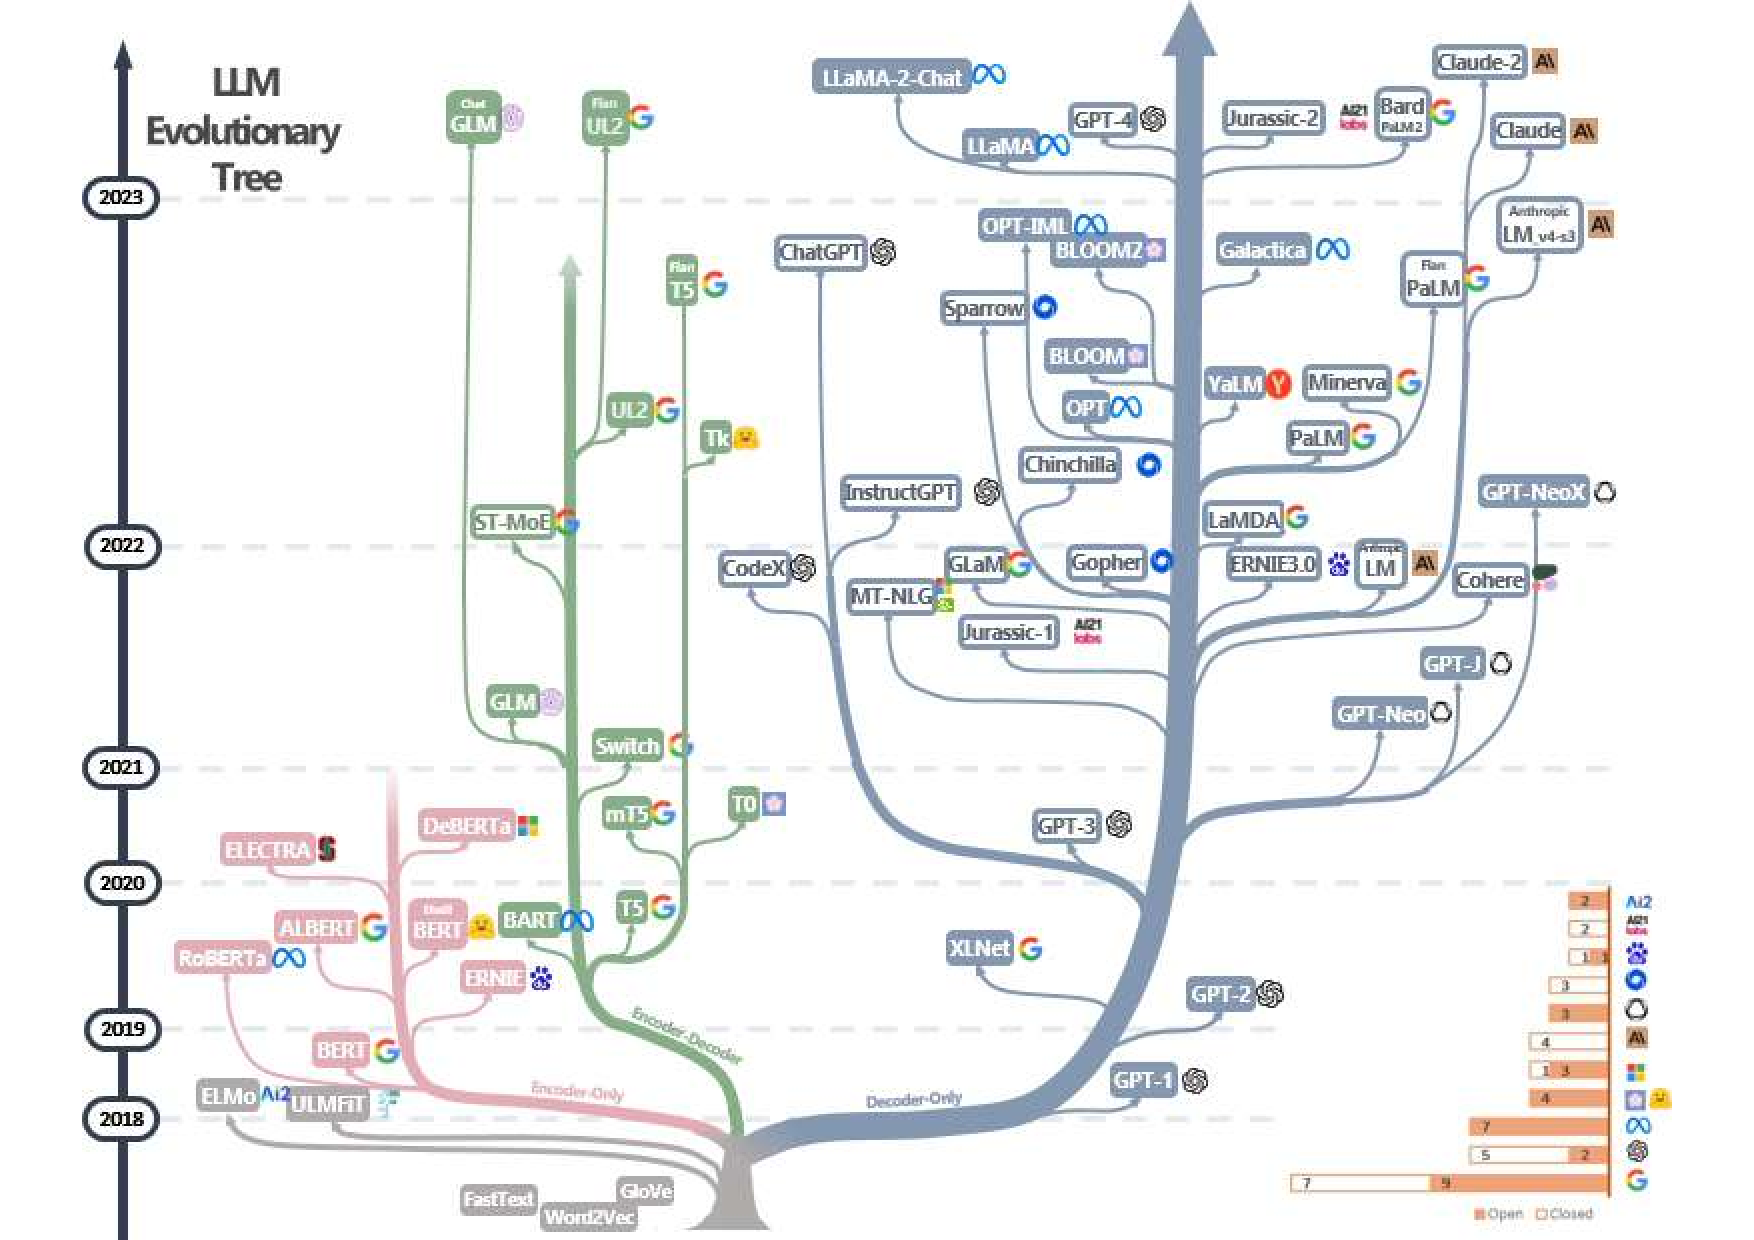
\includegraphics[width=1\textwidth]{Imagenes/treeLLM}
	\caption{Desarrollo de los LLM por\cite{yang2023harnessing}}
	\label{fig:3.1}
\end{figure}

Por un lado, el grupo ``solo codificador'', mostrado en rosa en la figura \ref{fig:3.1} incluye LLM que son buenos para la comprensión del texto porque permiten que la información fluya en ambas direcciones del texto. En azul, podemos ver el grupo ``solo decodificador'' que incluye LLM que son buenos en la generación de texto porque la información solo fluye de izquierda a derecha del texto para generar nuevas palabras de manera eficiente y autorregresiva. Finalmente, hay un tipo codificador-decodificador (mostrado en verde) que combina ambos aspectos y se usa para tareas que requieren comprender una entrada y generar una salida, como la traducción. 

Dentro de este último grupo encontramos la mayoría de los modelos que fueron considerados para el desarrollo de este trabajo como los distintos modelos de GPT, los de Google (Bard, que evolucionó a Gemini, LaMDA o PaLM).
\subsection{BERT}
Los modelos de lenguaje enmascarados, como los Masked Language Models, enmascaran un cierto porcentaje de palabras en una oración y se espera que el modelo prediga esas palabras en función del contexto restante \cite{rothman2022}. Un ejemplo representativo de este enfoque es BERT.

BERT (\textit{Bidirectional Encoder Representations from Transformers}) es un modelo de lenguaje enmascarado basado en la arquitectura Transformer \cite{devlin2019bert}. Desarrollado por Google en 2018, BERT ha demostrado un rendimiento sobresaliente en una variedad de tareas de procesamiento de lenguaje natural.

BERT se pre-entrena en dos grandes corpus de texto en inglés sin etiquetar: BookCorpus \cite{zhu2015aligning} y Wikipedia. Estos corpus garantizan una amplia cobertura de datos y una buena calidad para el entrenamiento del modelo.

Aunque inicialmente no estaba diseñado para la generación de texto, BERT ha sido adaptado para esta tarea, logrando mejoras significativas en comparación con modelos como GPT-2 \cite{wang2019bert}.

Existen numerosas variantes de BERT, algunas pre-entrenadas en dominios específicos y otras con un ajuste fino para tareas específicas \cite{rajasekharan2019review}. Por ejemplo, Beto es la versión en español de BERT, entrenada en un corpus extenso en dicho idioma \cite{canete2020spanish}.

La innovación clave de BERT es su enfoque bidireccional, que permite al modelo comprender el contexto de una palabra en función de su entorno completo. A diferencia de modelos unidireccionales como GPT-2, BERT considera tanto el contexto anterior como el posterior a una palabra dada.

La arquitectura de BERT consiste en una pila de codificadores de transformadores, con un número variable de capas dependiendo de la versión del modelo. Este enfoque permite a BERT realizar múltiples tareas de procesamiento de lenguaje, incluyendo Modelado de Lenguaje Enmascarado y Predicción de la Siguiente Oración \cite{devlin2019bert}.		


\subsection{T5}

T5, o Text-to-Text Transfer Transformer \cite{T5}, es un marco unificado para el aprendizaje por transferencia en procesamiento de lenguaje natural (PLN). Este enfoque revolucionario convierte todos los problemas basados en texto en un formato de texto a texto, donde el modelo recibe texto como entrada y genera nuevo texto como salida. Inspirado en marcos anteriores para tareas de NLP, como la modelización de lenguaje o la extracción de fragmentos, T5 permite aplicar el mismo modelo, objetivo de entrenamiento, procedimiento de entrenamiento y proceso de decodificación a cada tarea considerada.

El objetivo principal de T5 es proporcionar una perspectiva exhaustiva sobre el estado actual del campo de la transferencia de aprendizaje para PLN. En lugar de proponer nuevos métodos, se enfoca en la exploración y comparación empírica de técnicas existentes. Además, para facilitar futuros trabajos en este campo, se liberan conjuntos de datos, modelos pre-entrenados y código fuente.

\begin{figure}[h]
	\centering
	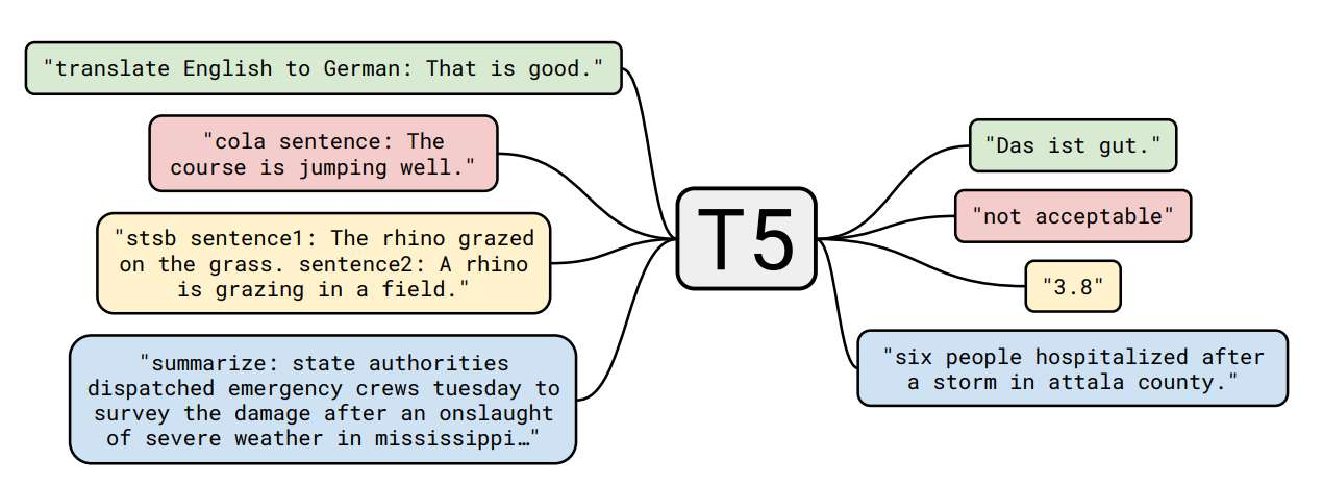
\includegraphics[width=0.9\textwidth]{Imagenes/T5}
	\caption{Diagrama del modelo T5 de \cite{T5}}
	\label{fig:3.2}
\end{figure}

Cómo se puede ver en la figura \ref{fig:3.2} el modelo T5 nos permite realizar diversas tareas como la traducción o la realización de resumenes.
%completar con las otras tareas que nos permite hacer no identifico que hace en lo rojo y amarillo 

\subsection{GPT (Generative Pretrained Transformer)}

Los modelos de lenguaje informales, también conocidos como modelos de lenguaje generativos, se centran en predecir palabras o tokens enmascarados dentro de una oración. Visualicemos un token enmascarado como un espacio en blanco dentro de una frase. En este escenario, el modelo solo considera el contexto anterior (palabras a la izquierda) y no tiene en cuenta el contexto posterior. La dirección del procesamiento no es crucial, siempre y cuando siga una dirección única, utilizando sólo las palabras relevantes del contexto para hacer predicciones, mientras descarta el resto. Esta propiedad clave de los modelos se refleja en su esquema de entrenamiento \citep{rothman2022}.

\subsubsection{GPT-1}

GPT-1 (Generative Pre-trained Transformer 1) fue el primer gran modelo de lenguaje desarrollado por OpenAI tras la introducción de la arquitectura Transformer por Google en 2017. En junio de 2018, OpenAI publicó un artículo titulado ``Improving Language Understanding by Generative Pre-Training'' \citep{radford2018improving}, donde presentaron este modelo inicial junto con el concepto general de un Transformer generativo pre-entrenado.

Hasta ese momento, los modelos de procesamiento de lenguaje neuronal con mejor desempeño se basaban principalmente en el aprendizaje supervisado a partir de grandes conjuntos de datos etiquetados manualmente. Esta dependencia limitaba su utilidad en conjuntos de datos poco etiquetados y hacía que el entrenamiento de modelos extremadamente grandes fuera costoso y lento. Muchos idiomas (como el suajili o el criollo haitiano) resultaban difíciles de abordar debido a la escasez de datos disponibles para la construcción de corpus. En contraste, el enfoque ``semi-supervisado'' de GPT implicaba dos etapas: una etapa de pre-entrenamiento generativo no supervisado, donde se establecían los parámetros iniciales mediante un objetivo de modelado de lenguaje, y una etapa de ajuste fino discriminatorio supervisado, donde estos parámetros se adaptaban a una tarea específica.

La elección de la arquitectura Transformer, en lugar de técnicas anteriores basadas en redes neuronales con atención mejorada, dotó a los modelos GPT de una memoria más estructurada que la alcanzada mediante mecanismos recurrentes, lo que resultó en un sólido desempeño en transferencia a diversas tareas.

\subsubsection{GPT-2}

GPT-2 es uno de los modelos más emblemáticos de lenguaje casual que sigue la arquitectura Transformer basada en auto-atención (masked self-attention). Presentado por OpenAI en 2019, fue aclamado desde el principio en el campo del Procesamiento de Lenguaje debido a su gran escala, con más de 1.5 billones de parámetros.

El objetivo principal de este sistema es construir una distribución de probabilidad donde cada posible palabra a generar recibe una probabilidad en función del contexto anterior. Este modelo fue pre-entrenado en un gran corpus de texto inglés utilizando el método auto-supervisado (self-supervised). Su propósito fundamental es la predicción de la siguiente palabra en una secuencia de palabras u oraciones.

Para el pre-entrenamiento, se creó un conjunto de datos llamado WebText, obtenido al extraer millones de páginas web a partir de enlaces de salida de Reddit que cumplían con ciertos criterios de calidad. Las páginas de Wikipedia asociadas a estos enlaces fueron excluidas. El resultado fue un corpus masivo de 40GB de textos adaptados para el entrenamiento de este modelo \citep{radford2019language}.

La estructura de GPT-2 se asemeja a la del Transformer original. Inicialmente, el modelo constaba de un codificador y un decodificador diseñados para tareas específicas como traducción automática. Sin embargo, GPT-2 abandonó esta arquitectura convencional y optó por una serie exclusiva de decodificadores basados en el Transformer. El número de decodificadores utilizados varía según el tamaño de GPT-2: desde doce en la versión Small hasta cuarenta y ocho en la versión Extra Large. Esta configuración basada únicamente en decodificadores es una característica distintiva de GPT-2, ilustrada en la Figura \ref{fig:gpt2_architecture}.

\begin{figure}
	\centering
	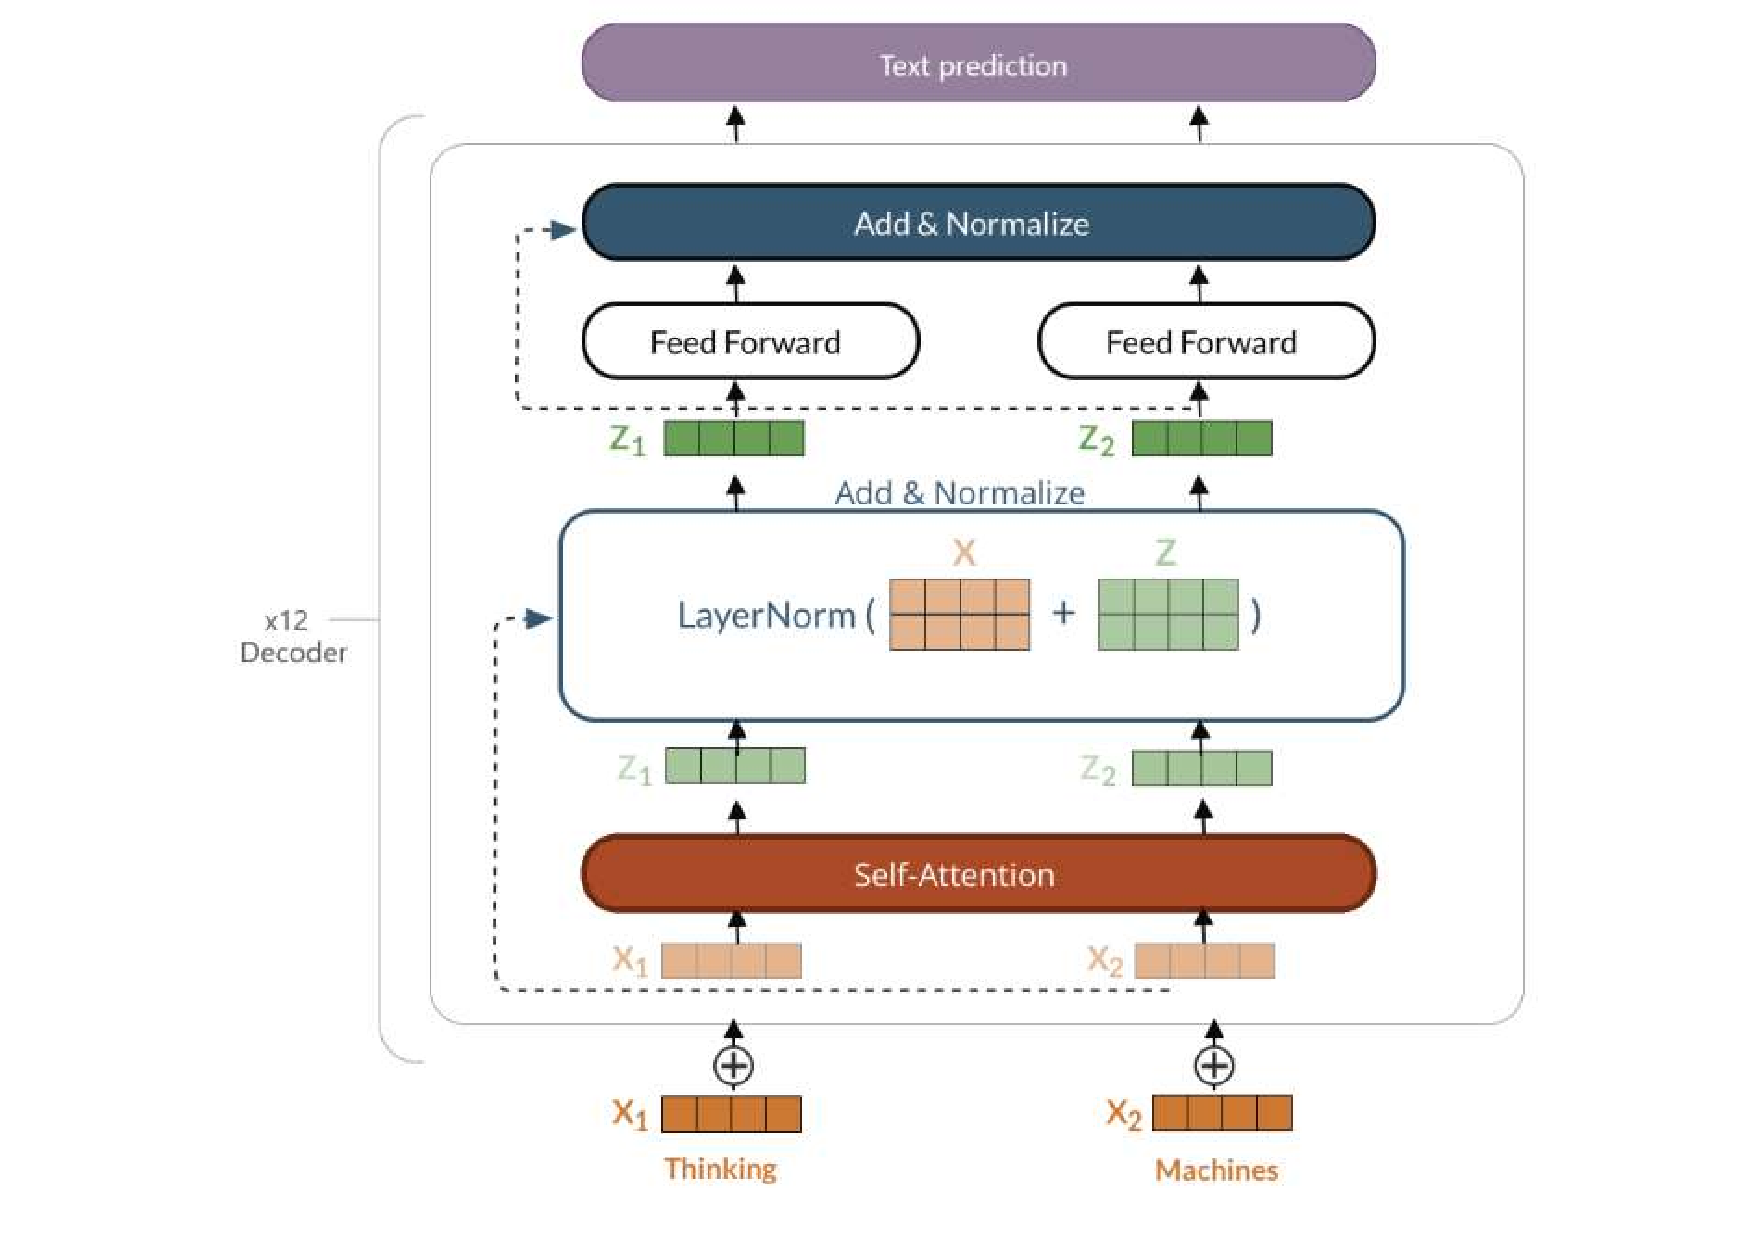
\includegraphics[scale=0.5]{Imagenes/gpt2_architecture}
	\caption{Arquitectura de GPT-2}
	\label{fig:gpt2_architecture}
\end{figure}

\subsubsection{GPT-3}

GPT-3 aumentó significativamente la cantidad de parámetros en comparación con GPT-2, alcanzando hasta 175 mil millones, lo que permitió una mayor complejidad y capacidad de aprendizaje. Gracias a su mayor capacidad y tamaño de conjunto de datos, GPT-3 demostró una mejor habilidad para generalizar y comprender una variedad más amplia de contextos y tareas. Además, requiere menos entrenamiento adicional para tareas específicas en comparación con GPT-2.

Por otro lado, a pesar de su mayor capacidad, GPT-3 logró reducir la generación de texto tóxico en comparación con GPT-2, aunque todavía se necesitaron estrategias de mitigación.

GPT-3 produce textos con mayor precisión y coherencia, lo que resulta en una calidad general de generación de texto más alta y una capacidad para realizar tareas más complejas.

\subsubsection{GPT-4}

GPT-4,\citep{GPT4} es el siguiente modelo de gran escala de OpenAI capaz de aceptar entradas de imagen y texto para producir salidas de texto. Aunque menos capaz que los humanos en muchos escenarios del mundo real, GPT-4 exhibe un rendimiento a nivel humano en diversos puntos de referencia profesionales y académicos, incluida la aprobación de un examen simulado de abogacía con una puntuación aproximadamente un 10$\%$ superior a la media de los examinados humanos. GPT-4 es un modelo basado en Transformers preentrenado para predecir el siguiente token en un documento. El proceso de ajuste posterior al entrenamiento mejora su rendimiento en medidas de factualidad y adherencia al comportamiento deseado.

En una serie de benchmarks tradicionales de Procesamiento de Lenguaje Natural (NLP), GPT-4 supera tanto a modelos de lenguaje grandes anteriores como a la mayoría de los sistemas de vanguardia (que a menudo requieren entrenamiento específico para el benchmark o ingeniería manual). En el benchmark MMLU, que cubre 57 temas en inglés, GPT-4 no solo supera a los modelos existentes en inglés, sino que también demuestra un rendimiento sólido en otros idiomas.

A pesar de sus capacidades, GPT-4 tiene limitaciones similares a modelos anteriores, como la falta de fiabilidad completa, una ventana de contexto limitada y la incapacidad de aprender de la experiencia. Las capacidades y limitaciones de GPT-4 plantean desafíos de seguridad significativos y novedosos..

\subsection{Llama}
A diferencia de la creencia común de que más parámetros conducen a un mejor rendimiento, investigaciones recientes muestran que modelos más pequeños entrenados con más datos pueden superar a los modelos más grandes. Se ha desarrollado una serie de modelos llamados LLaMA, \cite{touvron2023llama} que van desde 7B hasta 65B de parámetros, con un rendimiento competitivo en comparación con los mejores LLMs existentes.

Por ejemplo, LLaMA-13B supera a GPT-3 en la mayoría de las pruebas, a pesar de ser 10 veces más pequeño. Se espera que estos modelos democratizen el acceso y el estudio de los LLMs, ya que pueden ejecutarse en una sola GPU. Además, se asegura la compatibilidad con la fuente abierta al utilizar solo datos públicamente disponibles, a diferencia de otros modelos que dependen de datos no disponibles públicamente. El trabajo detalla las modificaciones realizadas en la arquitectura del $transformers$ \ref{sec:Transformers} y el método de entrenamiento, además de presentar el rendimiento de los modelos en comparación con otros LLMs en una serie de pruebas estándar. También se examinan los sesgos y la toxicidad codificados en los modelos, utilizando benchmarks de la comunidad de inteligencia artificial responsable.

El conjunto de datos de entrenamiento es una mezcla de varias fuentes, que cubren un conjunto diverso de dominios. Mayormente reutiliza fuentes de datos que se han utilizado para entrenar otros LLMs, con la restricción de utilizar solo datos públicamente disponibles y compatibles con la distribución abierta.

La tokenización de los datos se lleva a cabo con el algoritmo de codificación de bytes (BPE), utilizando la implementación de  $SentencePiece$ \footnote{El algoritmo $SentencePiece$ \cite{kudo2018sentencepiece} utiliza un enfoque basado en subpalabras, donde construye un vocabulario de subpalabras que se adaptan a la frecuencia de aparición en el corpus de entrenamiento. } . Dividimos todos los números en dígitos individuales y recurrimos a bytes para descomponer caracteres UTF-8 desconocidos. El tamaño total de nuestro conjunto de datos de entrenamiento contiene aproximadamente 1.4T de tokens después de la tokenización. La mayoría de los datos de entrenamiento se utilizan solo una vez durante el entrenamiento, con la excepción de los dominios de Wikipedia y Libros, sobre los cuales se realizan aproximadamente en dos épocas.
\subsection{Modelos LLM de Google AI}
A lo largo de los años Google AI ha desarrollado varios modelos LLM, todos ellos basados en Transformers, aunque con diferentes alcances y capacidades. A continuación se presentan estos modelos, aunque se explicaran con más profundidad a lo largo de la memoria. 
\subsubsection{LaMDA}
\label{sec:LaMDA}
LaMDA (Modelo de Lenguaje para Aplicaciones de Diálogo) fue el primer modelo LLM de Google AI. Su primera iteración fue anunciada durante la conferencia Google I/O de 2021, donde se presentó como un modelo conversacional de lenguaje. La segunda versión, presentada al año siguiente, introdujo mejoras y nuevas capacidades, como la generación de conversaciones originales sobre temas no previamente enseñados.

La atención sobre LaMDA aumentó cuando el ingeniero de Google, Blake Lemoine, afirmó que el chatbot se había vuelto sensible, lo que generó debates sobre la efectividad de la prueba de Turing para evaluar la inteligencia artificial general.

A diferencia de la mayoría de los modelos de lenguaje, LaMDA fue entrenado específicamente en diálogo. Durante su entrenamiento, adquirió sutilezas que distinguen las conversaciones abiertas de otras formas de lenguaje, como el sentido común.

La arquitectura Transformer utilizada por LaMDA es un modelo de solo decodificador, pre-entrenado en un corpus que incluye documentos y diálogos. Ha sido ajustado y probado con diferentes configuraciones de hiperparámetros, demostrando superar las respuestas humanas en ciertas áreas específicas.

\subsubsection{Bard}

Bard, anunciado por Google AI en 2022, se presenta como la evolución natural de su predecesor, LaMDA. Si bien este último ya destacaba por su capacidad para generar texto, traducir idiomas, escribir contenido creativo y responder a preguntas de forma informativa, Bard va un paso más allá. 

Bard se nutre de un conjunto de datos de texto y código aún más extenso que LaMDA, lo que le permite acceder y procesar información del mundo real a través de la Búsqueda de Google. Esto se traduce en respuestas más completas, precisas y actualizadas, ya que Bard se mantiene al día con los últimos acontecimientos y datos disponibles en la web. Su potencial creativo se expande a la escritura de diferentes tipos de contenido, desde poemas y código hasta guiones, piezas musicales, correos electrónicos y cartas. 

Además de la arquitectura Transformer, Bard incorpora otras técnicas de vanguardia como la atención y la decodificación autoregresiva. La atención permite a Bard centrarse en las partes más relevantes de un texto, mientras que la decodificación autoregresiva le permite generar texto palabra por palabra de forma coherente y fluida.

\subsubsection{Gemini}
Gemini es la última generación de modelos de lenguaje grandes de Google AI. Se anunció en 2024 y se basa en la arquitectura de Bard. Gemini es capaz de realizar todas las tareas que Bard puede hacer, y además tiene algunas características nuevas, como la capacidad de generar diferentes formatos de texto creativo, como poemas, código, guiones, piezas musicales, correo electrónico, cartas, etc. 

Su razonamiento multimodal avanzado le permite comprender y responder a preguntas complejas que involucran diferentes tipos de información, desde datos textuales hasta imágenes y vídeos. Gemini mejora constantemente sus habilidades y rendimiento a medida que se expone a nuevos datos y experiencias.

\section{Alucinaciones}
\label{sec:Alucinaciones}
En el campo de la inteligencia artificial (IA), se utiliza el término ``alucinación'' o ``alucinación artificiaL'' para describir respuestas de IA que no parecen estar justificadas por los datos de entrenamiento \cite{edwards2023chatgpt}. Este fenómeno, también conocido como confabulación o delirio, se refiere a la generación de respuestas o creencias que carecen de base sólida \cite{ji2022survey}. Por ejemplo, un chatbot alucinado podría ofrecer información falsa, como afirmar que los ingresos de Tesla fueron de 13.600 millones de dólares, un número aparentemente inventado \cite{lin2022trick}. Otros ejemplos de alucinaciones serían la generación respuestas inventadas como se puede ver en la imagen \ref{img:alucinacion}, donde ChatGPT genera un resumen de un artículo que no existe, o la adición de elementos en el estudio de imágenes, como se ve en la figura\ref{img:alucinacion2}.

\begin{figure}[h]
	\centering
	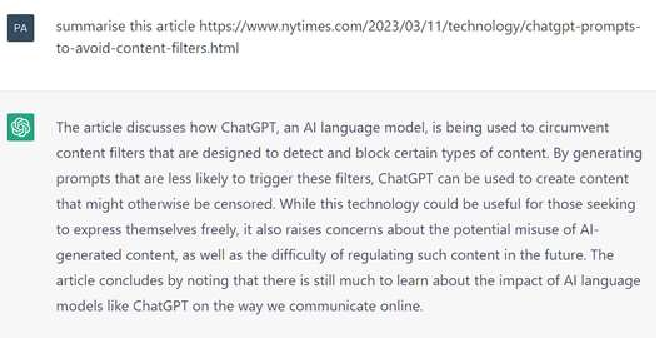
\includegraphics[scale=1]{Imagenes/ejemploAlucinacionGPT}
	\caption{Ejemplo de alucinación de ChatGPT \citep{wikialucinacion}}
	\label{img:alucinacion}
\end{figure}

\begin{figure}[h]
	\centering
	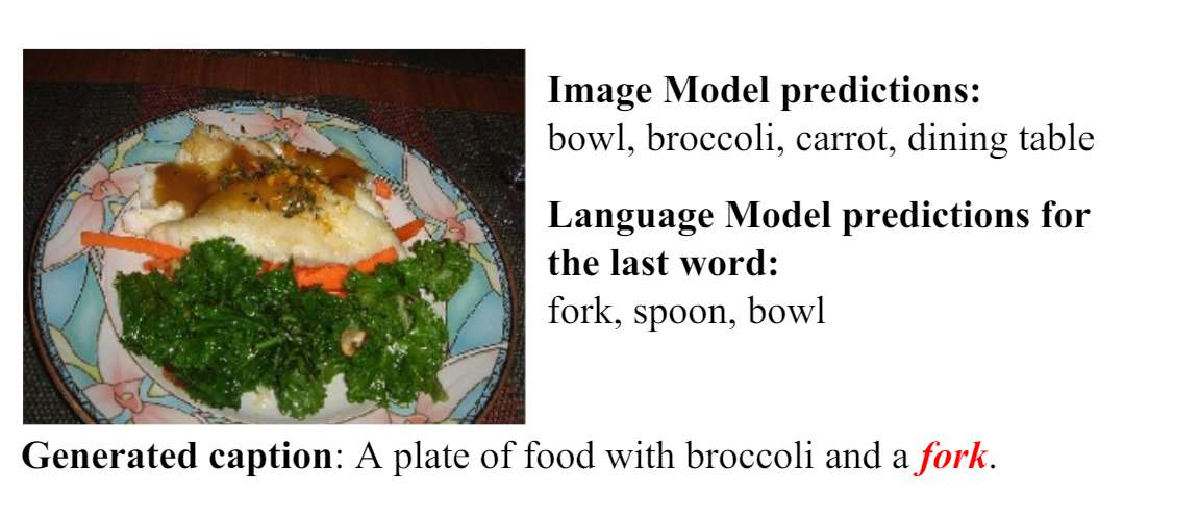
\includegraphics[scale=0.6]{Imagenes/alucinacionImagenes}
	\caption{Ejemplo de alucinación en una imagen \cite{rohrbach2023object}}
	\label{img:alucinacion2}
\end{figure}
Es importante destacar que, aunque se usa el término ``alucinación'' por analogía con la psicología humana, la diferencia fundamental radica en que las alucinaciones de IA se relacionan con respuestas injustificadas más que con percepciones falsas. Algunos investigadores señalan que este término antropomorfiza de manera poco razonable a los ordenadores.

El problema de las alucinaciones de IA se volvió prominente alrededor de 2022 con la introducción de modelos grandes de lenguaje como ChatGPT \citep{zhuo2023exploring}. Los usuarios expresaron preocupación por la capacidad de estos bots para insertar falsedades aparentemente plausibles en sus respuestas. En 2023, los analistas reconocieron las alucinaciones frecuentes como un desafío significativo en la tecnología de modelos de lenguaje \citep{leswing2023microsoft}.

Se cuestiona la confiabilidad del contenido generado por inteligencia artificial en el ámbito científico \citep{machinmastromatteo2023implicaciones}. Según Spinak (2023), los modelos de lenguaje de IA pueden percibir patrones que son imperceptibles para los humanos, lo que resulta en resultados inesperados o incorrectos, fenómeno conocido como ``alucinación'' \citep{spinak2023alucinaciones}. Estas alucinaciones pueden llevar a la producción de contenido falso, especialmente fuera de sus dominios específicos o al tratar con temas complejos o ambiguos, lo cual puede ser lingüísticamente plausible pero no científicamente preciso \citep{sage2023chatgpt}.

\section{Estado actual del procesamiento del lenguaje}
En los últimos años, el avance del procesamiento del lenguaje ha sido notable, con numerosas ventajas, aunque también con riesgos asociados al desarrollo de software.

Por un lado, los modelos de inteligencia artificial evolucionan rápidamente, generando frecuentes actualizaciones etiquetadas como ``última versión estable''. Esta denominación se refiere a la versión más reciente del modelo que ha sido probada y validada para su uso generalizado, ofreciendo calidad y fiabilidad.

Por otro lado, la IAs se enfrentan al problema de la regulación. La presidenta de la Comisión Europea, Ursula von der Leyen, ha subrayado que la IA está transformando nuestras vidas y ha enfatizado la importancia de un enfoque sensato y generalizado para beneficiar a la economía y la sociedad \citep{ComisionEuropea-ComunicadoPrensa-LeyIA}. La recién aprobada Ley de IA de la UE, considerada como el primer marco global en esta materia, busca promover la innovación responsable al regular los riesgos identificados y garantizar la seguridad y los derechos fundamentales de las personas y las empresas.

Este enfoque se basa en evaluar el riesgo de los sistemas de IA: aquellos de bajo riesgo, como los sistemas de recomendación, tendrán libertad y ninguna obligación, mientras que los de alto riesgo, como infraestructuras críticas, sistemas de salud y aplicaciones policiales, deberán cumplir requisitos estrictos de mitigación, calidad de datos y supervisión humana. Además, se prohibirán los sistemas de IA que representen una amenaza clara para los derechos fundamentales, como la manipulación del comportamiento humano. Se introducirán normas específicas para garantizar la transparencia en los modelos de IA de uso general, junto con multas para las empresas que no cumplan con las regulaciones.

En diciembre de 2023, se elaboró un borrador sobre la regulación de la IA por parte del Consejo de la Unión Europea y el Parlamento Europeo. Finalmente, el 2 de febrero de 2024, se aprobó la primera ley del mundo sobre inteligencia artificial: la Ley de IA. Después de una reunión en Bruselas, los embajadores de los 27 Estados miembros dieron su visto bueno político a esta normativa, tras la presentación en enero de la versión final del texto y la creación de la Oficina Europea de Inteligencia Artificial. Aunque algunos países mostraron oposición hasta el último momento, el camino continuó su curso y se prevé que entre 2024 y 2030 todos los países adopten la Ley de IA \citep{ElDerecho-LeyIA}.

Los constantes cambios en los modelos y las modificaciones en las legislaciones nacionales suponen un desafío para los desarrolladores de software. Durante el desarrollo de este proyecto, nos enfrentamos a diversas situaciones derivadas de estos sucesos. Por un lado, tuvimos que buscar una alternativa a la API de Bard, que se transformó en Gemini entre diciembre de 2023 y febrero de 2024, y por otro lado, hacer frente a las limitaciones impuestas por las diferentes leyes, que se solvento mediante el uso de VPN.

De hecho, la situación cambia tan rápidamente, que en la recta final del proyecto hemos observado varios cambios en los términos y condiciones de uso de la API de Gemini a nivel mundial. De hecho, la próxima actualización de los términos de uso será el 22 de mayo de 2024.

En conclusión, en el campo del desarrollo del lenguaje y la extracción de información a partir de imágenes, la IA está experimentando numerosos avances en los últimos años. Sin embargo, es fundamental tener en cuenta que el uso de los distintos modelos está sujeto a cambios tanto en las versiones y sus características, como en las leyes y términos y condiciones de uso.

\section{Otros trabajos relacionados}
\label{otrostrabajos}
\subsection{Proyecto Cantor}
El proyecto CANTOR (Composición automática de narrativas personales como apoyo a terapia ocupacional basada en reminiscencia) en el que se enmarca este trabajo, desarrolla herramientas digitales utilizando tecnologías de Inteligencia Artificial para construir automáticamente historias de vida que puedan ser reexaminadas posteriormente como apoyo a las terapias ocupacionales de pacientes con demencias.

CANTOR está financiado por el Ministerio de Ciencia e Innovación, en colaboración entre académicos de la Universidad Complutense de Madrid y la Universidad de La Coruña. El objetivo de CANTOR es desarrollar herramientas que faciliten la terapia ocupacional basada en reminiscencia para mejorar la calidad de vida de pacientes con deterioro cognitivo.

En este ámbito se han elaborado varios Trabajos de Fin de Grado en la Facultad de Informática de la UCM. Paso a referir algunos de ellos relacionados con este trabajo. 

\subsubsection{Generación de historias de vida usando técnias de Deep Learning}
\label{sec:trabajocristina}
En el curso 2021-2022, la compañera María Cristina Alameda Salas \citep{cristinaalameda}, en su trabajo de fin de grado, Generación de historias de vida
usando técnicas de Deep Learning, desarrolló un sistema basados en técnicas
de Deep Learning que de soporte a la generación de historias de vida. Partiendo de unos datos de entrada en forma de datos estructurados de tipo biográfico, ese trabajo permite la construcción de un sistema de generación de lenguaje natural, transformador de los datos de entrada a un escrito fluido y coherente, que abarque la representación de los datos de partida de manera completa, sin incorrecciones y lo más cercana posible a una redacción humana. Nuestro objetivo ahora sería el desarrollo de un programa que interactuara con el usuario y nos permitiera obtener toda esa información biográfica que da lugar a las historias de vida. 
\subsubsection{Extracción de preguntas a partir de imágenes para personas con problemas de memoria mediante técnicas de Deep Learning}

En 2021, en la UCM se desarrollo un trabajo de extracción de preguntas a partir de imagenes con técnicas de Deep Learning \citep{boto2021extraccion}. Este proyecto ayuda a las personas con problemas de memoria a recordar aspectos de su vida utilizando técnicas de IA como redes convolucionales y recurrentes. Para lograrlo se desarrolló un sistema capaz de extraer preguntas de fotografías que puedan representar recuerdos para las personas con problemas de memoria utilizando un bot que simula una sesión de terapia de reminiscencia.
El usuario ha de enviar fotografías al bot y este se encargará de enviarle, una a una, las preguntas generadas por la red neuronal. En este momento, el usuario deberá recordar todo lo posible sobre la imagen para poder responder a las preguntas y conseguir ejercitar su memoria.

\subsubsection{Extracción de información personal a partir de redes sociales para la creación de un libro de vida}
Este proyecto, desarrollado por \cite{aguilera2021extraccion}, tiene como objetivo principal ayudar a terapeutas ocupacionales en el tratamiento de pacientes con problemas de memoria, especialmente aquellos relacionados con el deterioro cognitivo asociado con la edad. Se propone la creación de una herramienta para desarrollar un libro de vida.

La herramienta combina técnicas de extracción y tratamiento de datos de diferentes redes sociales proporcionadas por el paciente, almacenándolos en una base de datos SQL para obtener la información más relevante. Esta información se utilizará para crear el libro de vida, que se presentará en una interfaz web desarrollada con React. La interfaz permitirá visualizar fácilmente los datos recopilados, utilizando tablas, mapas, líneas de tiempo y galerías de fotos.

\subsubsection{Generación de historias a partir de una base de conocimiento}
En este proyecto, desarrollado por \cite{lucia_latorre_magaz}, se construyó una aplicación para crear relaciones entre palabras e imágenes,
partiendo de unas palabras determinadas. Con las relaciones establecidas la aplicación genera estadísticas a través de las cuales puede evaluarse el progreso del paciente. En cada sesión se trata un tema concreto, pudiéndose elegir el tipo de sesión entre Sesión palabras (se elige una categoría de palabras), Sesión Progreso (se visualiza el avance del paciente a través de estadísticas agrupadas por categorías) o Sesión imágenes (donde se asocia una imagen a un concepto y una categoría).
\subsubsection{Recuerdame 1.0}
Recuerdame 1.0 \citep{recuerdame1.0} presenta la creación de una aplicación que facilite a los terapeutas la realización de terapias basadas en reminiscencia para tratar a pacientes con alzheimer, haciéndolas más ágiles y rápidas.

La aplicación creada es una aplicación web responsive, con una estructura Modelo Vista Controlador creada mediante lenguajes como HTML, CSS, PHP, JavaScript. La aplicación tiene una usabilidad aceptable, pero tiene detalles que mejorar y algunas funcionalidades que no pudieron ser desarrolladas por la falta de tiempo. 

\subsubsection{Recuerdame 2.0}
Durante el curso 2022-2023, la aplicación recuerdame 1.0 fue mejorada dando lugar a recuerdame 2.0 \citep{recuerdame2.0}, para ofrecer una experiencia terapéutica más enriquecedora a pacientes con problemas de memoria. Las mejoras incluyeron la optimización basada en la retroalimentación de usuarios finales, la narración mejorada de Historias de Vida, la generación automática de resúmenes, la integración de terapia con un bot, la mensajería entre terapeutas y cuidadores, y la capacidad de generar vídeos de Historias de Vida. Además, se realizó una evaluación exhaustiva del sistema en instituciones médicas y residencias de ancianos para validar su eficacia.

\subsection{Celia}

Celia, \footnote{\href{https://www.ambito.com/tecnologia/asi-es-celia-la-inteligencia-artificial-adultos-mayores-que-puede-detectar-indicios-alzheimer-n5921639}{Así es Celia, la inteligencia artificial para adultos mayores que puede detectar indicios de alzheimer}} es un chatbot impulsado por inteligencia artificial (IA) desarrollado por la compañía Atlantic, con el respaldo de la Xunta de Galicia en España. Este chatbot tiene como objetivo acompañar, entretener y brindar asistencia a las personas mayores y dependientes, y se destaca por su capacidad para detectar indicios y patrones de enfermedades neurodegenerativas, como el Alzheimer, mediante el análisis de la voz del usuario.

A diferencia de otros asistentes de conversación como Alexa o Siri, Celia va más allá al utilizar herramientas biométricas para medir y monitorear parámetros indicativos no solo de enfermedades neurológicas, sino también de condiciones emocionales como la ansiedad y la depresión.

Celia está disponible para su uso a través de tres plataformas: WhatsApp, la versión web y una aplicación oficial disponible actualmente solo para dispositivos Android. Los usuarios pueden interactuar con Celia a través de mensajes de texto o de voz, y la instalación es sencilla, lo que permite un acceso rápido y eficiente a este recurso tecnológico.

Una característica destacada de Celia es su capacidad para tomar la iniciativa en las conversaciones y proponer actividades sin necesidad de instrucciones. Además, ofrece la posibilidad de establecer recordatorios para citas médicas o la toma de medicamentos, brindando un apoyo integral en la gestión de la salud de los usuarios.
\section{Conclusión}
El procesamiento del lenguaje natural es un campo de las ciencias de computación que está experimentando una gran evolución gracias a los avances y la creciente popularidad de la IA. Elegir, de entre todas las técnicas de PLN existentes, aquellas que se adaptan más a nuestras necesidades, será crucial para simplificar el trabajo. 

En este capítulo, se ha mostrado en rasgos generales cuales son las distintas alternativas: desde las más sencillas hasta las más potentes. Por otro lado, estudiar otros trabajos relacionados (sección \ref{otrostrabajos}) nos advierte acerca de los retos a los que nos vamos a enfrentar. Además, nos permite descubrir herramientas e ideas que sirven de inspiración para el desarrollo de nuestro propio proyecto. 

Con la visión general que nos da el estudio realizado hasta el momento pasamos al capítulo \ref{cap:TecnologiasUtilizadas}. En él, estudiaremos en profundidad las herramientas concretas que se pretende usar y se valorará las mejores alternativas.
